\chapter{Wstęp}
\section{Wprowadzenie}


Rozpowszechnione algorytmy sztucznej inteligencji wspomagające pracę inżynierów dźwięku można podzielić na dwie główne dziedziny \cite{analysis_generative} \label{traditional_algos}:

\begin{enumerate}
    \item algorytmy generujące symboliczny zapis muzyki (nuty lub dane MIDI) (\ref{fig:lamus_notes}),
    \item algorytmy generujące gotowy plik audio (\ref{fig:riffusion_spectro}).
\end{enumerate}

Pierwsza grupa algorytmów znana jest już od lat 80, gdyż zagadnienie generowania zapisu symbolicznego jest mniej wymagające niż wytworzenie pełnego pliku audio.
Powszechnie wykorzystywana jest w nich teoria muzyki, pozwalająca określić matematyczne relacje w rytmach, melodiach i progresjach akordów.
Wiedza dotyczącą teorii muzyki pozwala na wyznaczenie możliwej przestrzeni stanów, w której generowana jest kompozycja,
natomiast modele matematyczne takie jak łańcuchy \textit{Markowa} służą za mechanizmy decyzyjne, które ,,nawigują'' w przestrzeni stanów.

\begin{figure}[H]
    \centering
    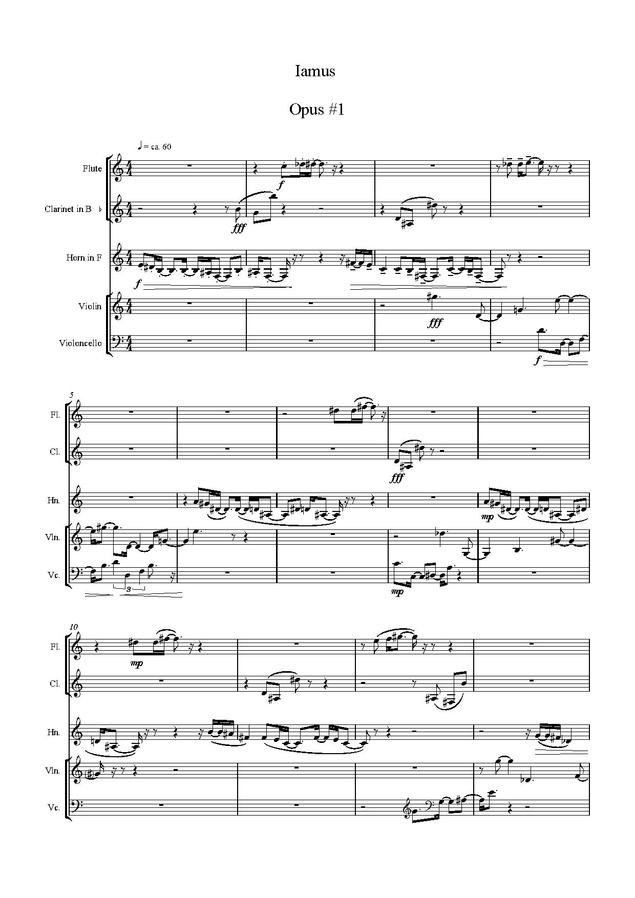
\includegraphics[width=0.4\linewidth]{rys01/lamus_notes.jpg}
    \caption{Zapis nutowy utworu \textit{Opus One}, wygenerowany przez komputer \textit{Lamus}.}
    \label{fig:lamus_notes}
\end{figure}

Druga grupa algorytmów, generująca pliki audio, rozwija się na bazie nowych możliwości,
które zapewniają algorytmy wywodzące się ze \textit{Stable Diffusion} \cite{stablediffusion}.
Najnowsze modele generujące pliki audio zgodne z opisem tekstowym 
(przykładowo   \texttt{,,smutny jazz''} bądź \texttt{,,muzyka taneczna w stylu Depeche Mode''})
szkolone są w taki sam sposób jak algorytmy stable diffusion. 
Jednakże zamiast na obrazach artystów, modele takie jak \textit{Stable Riffusion} \cite{riffusion} 
uczą się na spektrogramach, które następnie są w stanie wygenerować (\ref{fig:riffusion_spectro}).
Po wygenerowaniu spektrogramu przez model,
jest on konwertowany do pliku audio za pomocą odwrotnej transformaty Fouriera.

\begin{figure}[H]
    \centering
    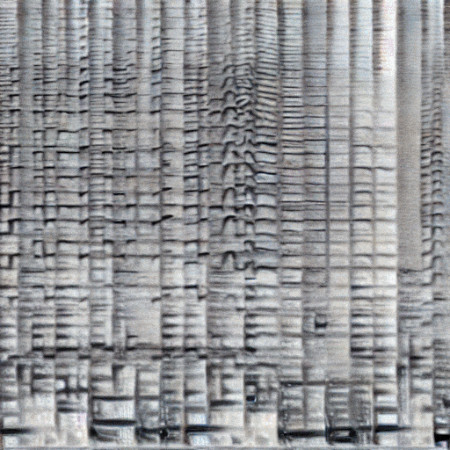
\includegraphics[width=0.4\linewidth]{rys01/riffusion_spectro.jpg}
    \caption{Przykładowy spektrogram wygenerowany przez algorytm \textit{Stable Riffusion} dla danych wejściowych \texttt{funk bassline with a jazzy saxophone solo}.}
    \label{fig:riffusion_spectro}
\end{figure}

% TODO: check later
% https://github.com/Kinyugo/msanii

Obie metody opisane w rozdziale~\ref{traditional_algos} można porównać pod względem ich przydatności
dla użytkownika końcowego, czyli osoby zajmującej się produkcją nagrań muzycznych. Metoda pierwsza, 
generowanie zapisu symbolicznego, może wydawać się mniej zaawansowana niż generowanie całych plików dźwiękowych.
Jednakże, z perspektywy użytkownika, zapis symboliczny jest bardziej praktyczny,
ponieważ możliwe jest zaimportowanie go do programu DAW i późniejsza modyfikacja zapisu nutowego.
Obecnie dostępne modele generujące pełne nagrania z muzyką nie umożliwiają
szczegółowego edytowania parametrów wygenerowanego dźwięku, ponieważ operują bardzo wysokopoziomowo 
-- syntezują muzykę na podstawie opisu słownego.

Niniejsza praca realizuje zadanie,
którego nie da się zaklasyfikować do żadnej z dwóch wyżej wymienionych (\ref{traditional_algos}) dziedzin.
Wynik pracy algorytmu implementowanego w ramach pracy magisterskiej jest \textbf{gotowym elektronicznym
instrumentem muzycznym}, który może być wykorzystany w programie do komponowania muzyki.
Tego typu proces generowania grafów przetwarzania sygnałów dźwiękowych może być porównany z procesem projektowania instrumentu muzycznego.

Proces dynamicznego modyfikowania grafu przetwarzania sygnału jest często wykorzystywany w muzyce
elektronicznej, do tworzenia dźwięków o interesującej barwie bądź dynamice. Syntezatory dźwięku
dostępne na rynku często wyposażone są w \textit{patch bay}, pozwalający na modyfikowanie
grafu przepływu sygnałów wewnątrz syntezatora, bądź połączenie go z zewnętrznym sprzętem muzycznym
bądź elektronicznym (\ref{fig:mother32}).

\begin{figure}[H]
    \centering
    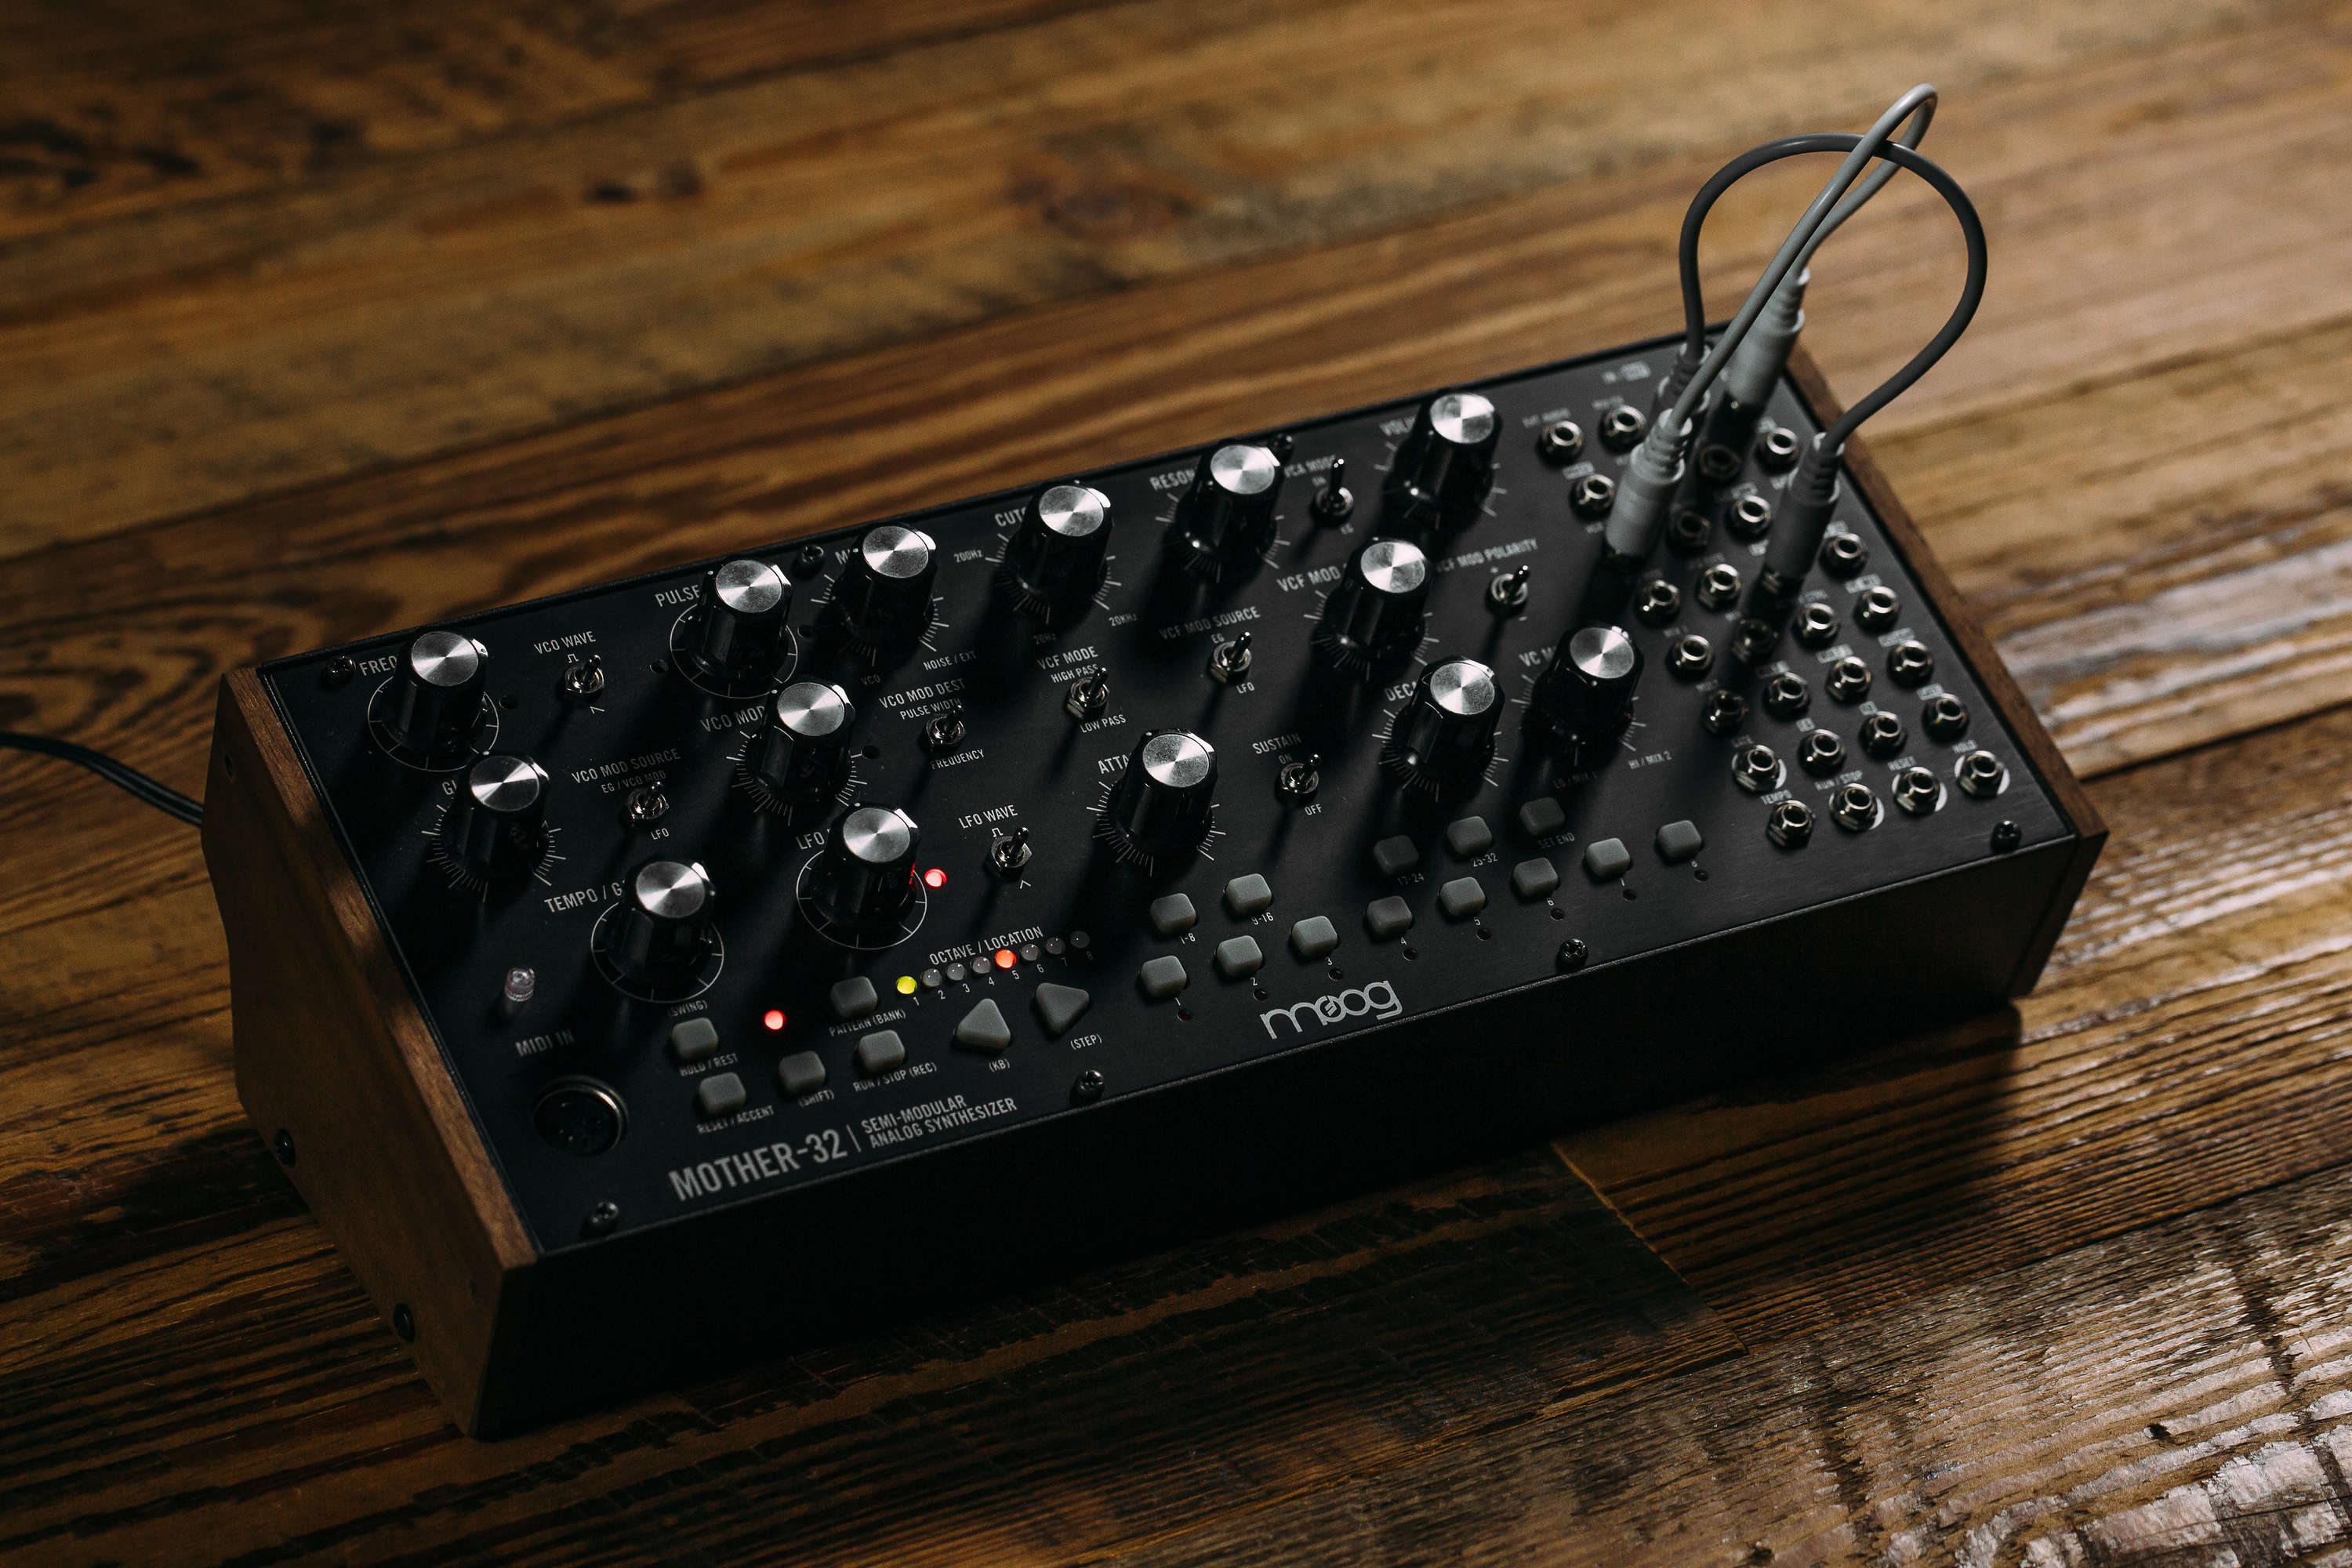
\includegraphics[width=0.7\linewidth]{rys01/mother32.jpg}
    \caption{Syntezator \textit{Mother 32} firmy \textit{Moog}, po prawej stronie widoczny
    jest \textit{patch bay} z podłączonymi przewodami, które zmieniają konfigurację
    połączeń między układami generującymi i przetwarzającymi sygnał dźwiękowy.}
    \label{fig:mother32}
\end{figure}


\section{Cel pracy}


Celem pracy jest zbadanie, czy algorytmy optymalizacyjne są w stanie
wytworzyć graf przetwarzania sygnałów audio, który wykona syntezę próbki
dźwięku zadanej przez użytkownika.
Problem poruszany w pracy można zakwalifikować do grupy zagadnień związanych
z pojęciem \textit{computer-aided design} w dziedzienie inżynierii dźwięku. Docelowo
zaimplementowany algorytm będzie automatyzował pracę inżyniera dźwięku,
tworząc i konfigurując grafy przetwarzania sygnałów dźwiękowych, dostępne w
programach typu \textit{digital audio workstation}~\ref{fig:ableton_patch}. Badania obejmują dwa zagadnienia:
\begin{enumerate} \label{research_types}
    \item metody generowania grafu przetwarzania sygnałów oraz późniejszej modyfikacji grafu,
    \item dobór funkcji celu, na podstawie której algorytm optymalizujący będzie przeszukiwał
możliwą przestrzeń grafów przetwarzania sygnałów.
\end{enumerate}

Pierwsze zagadnienie sprowadza się do przetestowania szeregu algorytmów pozwalających na wygenerowanie
grafu przetwarzania sygnałów DSP oraz ich modyfikację. Przykładem modyfikacji grafu
może być wprowadzanie w nim losowych zmian lub krzyżowanie dwóch grafów DSP w przypadku
wykorzystania algorytmu genetycznego.
Graf przetwarzania sygnałów można opisać jako zbiór połączonych węzłów generujących
i przetwarzających sygnał dźwiękowy. Każdy węzeł można opisać poprzez:

\begin{enumerate}
  \item zbiór wejść,
  \item zbiór wyjść,
  \item operację matematyczną, wykonywaną na sygnale.
\end{enumerate}

Pełny graf przetwarzania można opisać za pomocą zbioru węzłów oraz
macierzy połączeń między węzłami:

$N$ - liczba węzłów,

$i_{j} = [ p_1, p_2, \ldots, p_n ]$ -- Zbiór wejść (\textit{inputs}) j-go węzła,

$o_{j} = [ p_1, p_2, \ldots, p_n ]$ -- Zbiór wyjść (\textit{outputs}) j-go węzła,

$f_i(x)$ -- operacja wykonywana na sygnale przez i-ty węzeł.

$C = [ \{ o_{(j, k)}, i_{(l, m)} \}, \ldots ] $ -- zbiór połączeń między węzłami, opisujący, które 
$k$-te wyjście $j$-go węzła podłączone jest do którego $m$-go wejścia $l$-go węzła.

Nie wszystkie wejścia w grafie muszą wyć podłączone do któregoś z wyjść.
Wejście, które nie zostało nigdzie podłączone przyjmuje jako wartość parametr 
liczbowy optymalizowany później w funkcji celu~\ref{eq:target_function}.
W przypadku schematu~\ref{fig:minilogue_diagram} takimi ,,wolnymi'' wejściami są przykładowo
sygnał określający wysokość dźwięku oraz parametry określające parametry
generatora obwiedni~(\textit{EG}).


\begin{figure}[H]
    \centering
    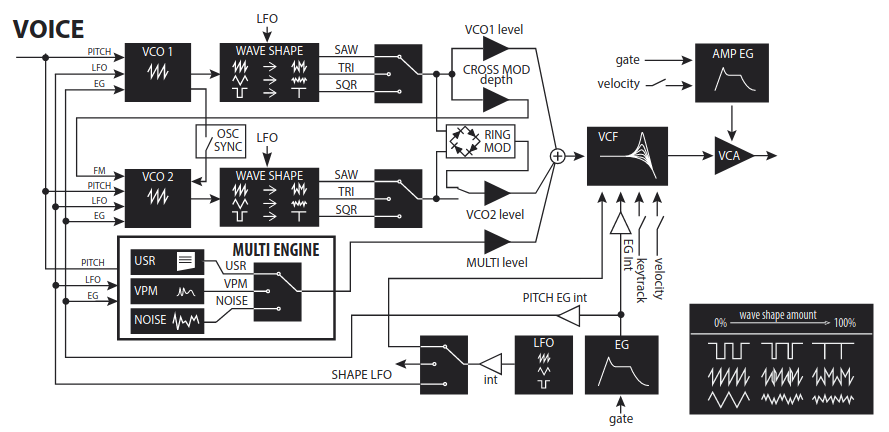
\includegraphics[width=0.8\linewidth]{rys01/minilogue_voice_block_diagram.png}
    \caption{
      Diagram blokowy pojedynczego głosu w syntezatorze 
      \textit{Minilogue xd} firmy \textit{Korg} \cite{minilogue_diagram}.
    }
    \label{fig:minilogue_diagram}
\end{figure}

Dla powszechnie wykorzystywanego w analogowych syntezatorach subtraktywnych 
schematu przetwarzania sygnałów~(\ref{fig:minilogue_diagram}) można wyróźnić przykładowe węzły: \\

\begin{multicols}{2}

\noindent
\textbf{Oscylator} (\textit{VCO}):
\begin{enumerate}
  \item Wejścia:
    \begin{itemize}
      \item częstotliwość,
      \item kształt fali.
    \end{itemize}
  \item Wyjścia:
    \begin{itemize}
      \item wygenerowany sygnał.
    \end{itemize}
\end{enumerate}

\noindent
\textbf{Filtr} (\textit{VCF}):
\begin{enumerate}
  \item Wejścia:
    \begin{itemize}
      \item częstotliwość odcięcia,
      \item rezonans.
    \end{itemize}
  \item Wyjścia:
    \begin{itemize}
      \item przefiltrowany sygnał.
    \end{itemize}
\end{enumerate}
\end{multicols}


Drugie zagadnienie obejmuje przetestowanie szeregu algorytmów, które można wykorzystać jako funkcję celu,
która będzie optymalizowana poprzez ,,dostrajanie'' grafu przetwarzania sygnałów dźwiękowych.

Funkcja celu, oceniająca, jak sygnał wygenerowany ($\bar{x}$) przez algorytm jest bliski sygnałowi docelowemu ($x$)
może zostać przedstawiona w następujący sposób:

\begin{equation}
  F(x, \bar{x}) = q
  \label{eq:target_function}
\end{equation}

Następnie, dla danego układu $N$ węzłów przetwarzania oraz dla macierzy połączeń $C$, 
należy rozwiązać następujący problem optymalizacji, należy rozwiązać problem
maksymalizacji funkcji opisanej równaniem~\ref{eq:target_function} dla
parametrów wszystkich wejść $i_j$ oraz $o_j$, które nie są połączone bezpośrednio
pomiędzy węzłami.

\begin{figure}[H]
    \centering
    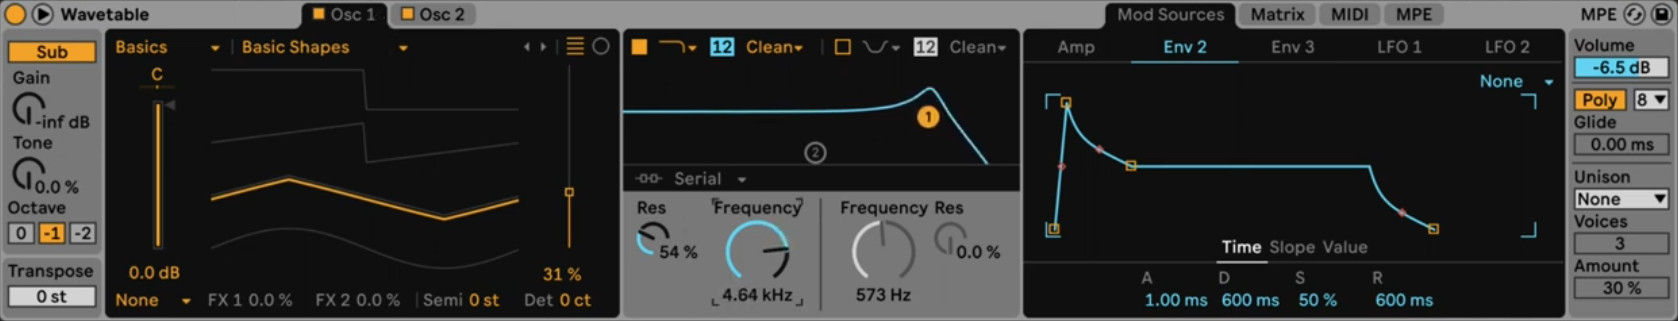
\includegraphics[width=0.8\linewidth]{rys01/ableton_patch.jpg}
    \caption{
      Zbiór parametrów konfigurujących przykładowy syntezator dźwięku w programie \textit{Ableton}}
    \label{fig:ableton_patch}
\end{figure}


\section{Zakres pracy, plan badań}

\subsection{Metody generowania grafu przetwarzania sygnałów oraz późniejsza modyfikacja grafu}

Głównym problemem przy generowaniu grafu przetwarzania sygnałów są ograniczenia nałożone na strukturę grafu,
które należy spełnić, by graf był logicznie interpretowalny jako łańcuch przetwarzania sygnałów.
Graf musi być grafem skierowanym, który nie zawiera pętli o dodatnim sprzężeniu zwrotnym 
(lub nie zawiera ich wcale, co można założyć dla uproszczenia problemu).
Struktura grafu powinna być możliwie jak najbardziej przejrzysta dla użytkownika. 
Automatyczna ewolucja może dążyć w kierunku wykorzystania nadmiarowej liczby
bloków przetwarzania sygnału, jeśli funkcja celu nie będzie zawierała kary za zbyt złożone grafy.
Podobne prace \cite{evolutionary_puredata} wykorzystują podejście oparte o 
\textit{mixed-typed carthesian genetic programming}, które będzie punktem startowym dla pracy.
Finalnie, badania dążą do wyznaczenia algorytmu o następujący właściwościach:

\begin{enumerate}
    \item algorytm generuje grafy będące logicznie spójnymi łańcuchami przetwarzania dźwięku (skierowany, bez pętli o dodatnim sprzężeniu zwrotnym w natężeniu sygnału),
    \item algorytm maksymalizuje wykorzystanie poszczególnych bloków przetwarzania w grafie, co minimalizuje finalny rozmiar grafu, czyniąc go bardziej czytelnym,
    \item generowany graf posiada reprezentację umożliwiającą wykonanie krzyżowania dwóch grafów przetwarzania sygnału. Graf będący wynikiem krzyżowania nadal musi być poprawnym grafem przetwarzania sygnału.
\end{enumerate}

Elementami grafu przetwarzania sygnałów są używane powszechnie w syntezie dźwięku algorytmy:

\begin{enumerate}
  \item modulacja FM \cite{spectral_audio_processing} \cite{computational_music_synthesis},
  \item synteza subtraktywna \cite{computational_music_synthesis} \cite{digital_filters},
  \item algorytmy \textit{physical modeling} \cite{lisp_synthesis} \cite{computational_music_synthesis},
  \item symulacja efektu pogłosu/echa \cite{reverb} \cite{freeverb}.
\end{enumerate}

\subsection{Dobór funkcji błędu -- różnica między wygenerowanym a docelowym sygnałem dźwiękowym}

Funkcja celu poszukiwana w ramach projektu musi określać, jak dobrze sygnał wygenerowany przez
graf przetwarzania sygnałów pokrywa się z sygnałem docelowym. Porówanie sygnałów musi skupiać się
na cechach sygnału, które są najbardziej słyszalne dla ludzkiego ucha. Jednocześnie funkcja nie powinna
,,karać'' sygnałów, które są względem siebie przesunięte w fazie. Wśród algorytmów, które zostały wybrane
do przetestowania w ramach projektów zawarte są:

\begin{enumerate}
  \item algorytmy porównywania sygnałów oparte o transformatę Fouriera~\cite{sliding_fourier} \cite{mfcc},
  \item techniki wykorzystywane do generowania ,,cyfrowych podpisów'' sygnałów dźwiękowych (\textit{sound fingerprinting}) \cite{computer_vision_music_identification},
  \item algorytmy wykrywające spadek jakości dźwięku z perspektywy psychoakustycznej \cite{peaq} \cite{frechet_audio_distance}.
\end{enumerate}

